\documentclass[11pt]{article}
\usepackage[italian]{babel}
\usepackage[utf8]{inputenc}

\usepackage{titlepic} % redefines the \maketitle command to include a picture on your title page, that you provide via the \titlepic command
\usepackage{natbib}
\usepackage{graphicx}
\usepackage{hyperref}
\hypersetup{
    colorlinks=true,
    linkcolor=black,        % color of internal links           %% Andrea
    citecolor=black,        % color of links to bibliography    %% Andrea
    filecolor=blue,         % color of file links               %% Andrea
    urlcolor=blue,          % color of external links           %% Andrea
}

\title{Progetto Interazione Uomo Macchina}
\date{A.A. 2019/2020}
\setcounter{page}{0}

\makeatletter
\def\projectName{Beni culturali}
\let\documentTitle\@title    
\let\academicYear\@date
\makeatother

\begin{document}
\begin{titlepage}
	\centering
    \vspace*{0.5 cm}
    
\includegraphics{images/logosapientini.png}\\[0.75 cm]
%    \textsc{\large Progetto Interazione Uomo Macchina}\\[0.5 cm]
	\textsc{\textit{Università La Sapienza}, Informatica}\\[0.25 cm]
	\textsc{\academicYear}\\[0.5 cm]
	\rule{\linewidth}{0.2 mm} \\[0.4 cm]
	\textsc{\large \documentTitle}\\[0.4 cm]
	%\rule{\linewidth}{0.2 mm} \\[0.4 cm]
	\textsc{\Huge \projectName}\\
	\rule{\linewidth}{0.2 mm} \\[1.5 cm]
	
	\large
	Alessio Berardi, 1796857\\[0.2 cm]
	Andrea Gasparini, 1813486\\[0.2 cm]
    Edoardo Di Paolo, 1728334\\[0.2 cm]
    Enrico Graziani, 1806141\\[0.2 cm]
    Riccardo La Marca, 1795030\\[0.2 cm]
\end{titlepage}

\tableofcontents
\pagebreak

\section{Introduzione}

Questo documento contiene la relazione relativa al progetto del gruppo \textit{Sapientini Dream Team} per il corso di \textit{Interazione Uomo-Macchina}, tenuto dal professor Emanuele Panizzi.

\paragraph{}
Il tema del progetto sono i \textit{Beni Culturali}, più nello specifico i \textbf{Musei} e le \textbf{Mostre} di \textbf{Roma}, e la piattaforma di riferimento scelta per il prototipo è \textit{Android}. 

\paragraph{A cura di:}
\begin{itemize}
    \item Alessio Berardi
    \item Andrea Gasparini
    \item Edoardo Di Parolo
    \item Enrico Graziani
    \item Riccardo La Marca
\end{itemize}
\pagebreak

\input{documents/needfinding/appsimili.tex}
\pagebreak

\section{Needfinding}
\def\people{20}

\section{Interviste}

\subsection{Introduzione}
Questa sezione riassume i risultati che si sono evinti dalle interviste che abbiamo svolto. Il numero totale di intervistati è di \textbf{\people} persone. Questa fase è stata divisa in due parti poiché ci siamo resi conto che le prime interviste coprivano un campo troppo generico che abbiamo quindi ristretto. I risultati nel dettaglio si riferiscono alle sole informazioni utili raccolte durante la prima fase e a tutte quelle della seconda.

\paragraph{}
Per rendere più efficiente la fase delle interviste abbiamo deciso di dividerci in due gruppi, uno da 2 persone e l'altro da 3 persone, affinché in ogni gruppo ci fosse almeno una persona che aveva come compito quello di prendere appunti riguardo le risposte dateci dagli intervistati.

\subsection{Risultati nel dettaglio}
Andando nel dettaglio, nelle interviste abbiamo toccato, principalmente, i seguenti temi:
    \begin{itemize}
      \item acquisto biglietti (\textit{solo prima fase});
        \item frequenza di visite a musei;
        \item ricerca di informazioni riguardanti musei da visitare;
        \item informazioni riguardanti l'utilizzo o meno delle visite guidate;
        \item informazioni riguardanti sconti universitari (incluse le domeniche gratuite);
        \item informazioni riguardanti l'utilità delle recensioni.
    \end{itemize}
    
\paragraph{}    
Abbiamo chiesto subito come venissero a conoscenza dei musei da visitare e abbiamo scoperto che la maggior parte delle persone si informa grazie ai cartelloni pubblicitari esposti in \textbf{metropolitana, autobus, strade e volantini}. Ovviamente, oltre a questa tipologia di pubblicità, c'è quella che avviene sui \textbf{Social Network}. Relativamente invece all'acquisto dei biglietti si è scoperto che molti li acquistano online in maniera da evitare la fila, invece il restante alla vecchia maniera: cioè al botteghino. In quest'ultimo caso gli intervistati non avevano problemi ad attendere il proprio turno.

\paragraph{}
La maggior parte degli intervistati ha detto di preferire un'\textbf{audioguida} alle \textbf{visite guidate}. Addirittura in molti hanno ammesso di informarsi autonomamente poiché la visita, altrimenti, sarebbe costata di più.
\newline
Gli \textbf{sconti universitari} vengono utilizzati dalla quasi totalità degli studenti intervistati, riguardo le \textbf{domeniche gratuite} invece, la maggior parte ha ammesso di voler utilizzare questa offerta ma, a causa del flusso esagerato di persone, ci rinunciano nella maggior parte dei casi.

\paragraph{}
Le eventuali recensioni di un museo non influenzano la voglia di visitarlo per la maggior parte delle persone. Tutti gli intervistati hanno ammesso di non lasciare alcuna recensione dopo la visita.



\pagebreak
\def\answers{257}

\subsection{Questionario}

Questa sezione riassume i risultati che abbiamo ricevuto dalle risposte al \href{https://docs.google.com/forms/d/1vKzFGCQb5nvyG6it8HfEqZgZ3ioQ6J1_T6eUiTdYIRc/edit}{questionario}. 
Prima di condividere il questionario, abbiamo effettuato un test \textbf{pilota} con 5 utenti per assicurarci che non ci fossero problemi o parti ambigue. Il numero finale di risposte ricevute al questionario è pari a \textbf{\answers}.

\subsubsection{Risultati}
Ai fini del questionario abbiamo raccolto informazioni statistiche, in particolare età e attuale posizione lavorativa. Dai risultati, il \textbf{45\%} è risultato essere studente, il \textbf{34\%} lavoratore, il \textbf{12\%} è studente-lavoratore e il rimanente è disoccupato. Per quanto riguarda l'età, il \textbf{53\%} ha tra i 18-25 anni, il \textbf{19\%} tra i 26 e i 35, l'\textbf{8\%} è minorenne e il restante \textbf{20\%} ha un'età superiore ai 50 anni.

\paragraph{}
Abbiamo scoperto che la metà degli intervistati visita i musei almeno una volta all'anno, mentre solamente in 4 hanno detto di visitarne almeno uno alla settimana.\\
Le visite guidate, dalle risposte, sembrano essere apprezzate e risultano essere utili. 
Si è scoperto che le persone preferiscono andare a visitare un museo in compagnia piuttosto che da soli, ma dalle risposte abbiamo capito che la maggior parte delle persone non trova interessante, o importante, ciò che i propri amici hanno visitato di recente, anche se allo stesso tempo hanno trovato molto utile la possibilità di organizzare visite di gruppo con essi attraverso l'utilizzo dell'applicazione.

\begin{figure}[ht]
    \centering
    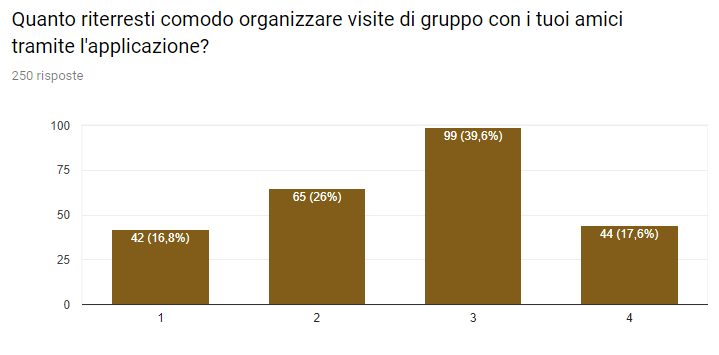
\includegraphics[width=1.0\textwidth]{images/charts-questionario/chart-visite-gruppo.png}
\end{figure}

\begin{figure}[ht]
    \centering
    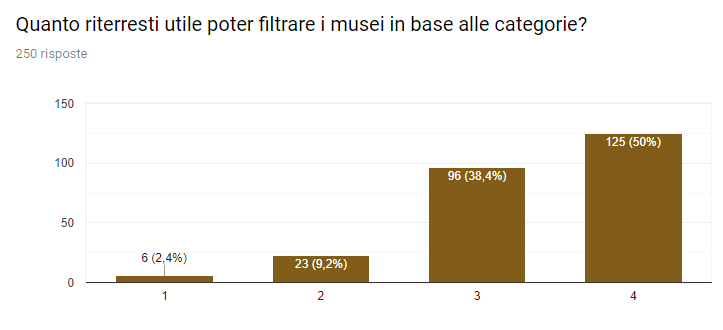
\includegraphics[width=1.0\textwidth]{images/charts-questionario/chart-filtro-categorie.png}
\end{figure}

\paragraph{}
La cosa davvero utile, a quanto pare, è la possibilità di filtrare i musei in base alle categorie che ci sono state segnalate nelle altre risposte.\\
Per quanto riguarda le recensioni, più dell'\textbf{80\%} ha detto di non rilasciarne dopo una visita, anche se comunque la scelta di visitare una mostra rispetto ad un'altra viene molto influenzata dalle recensioni della stessa. Infatti per il \textbf{54\%} delle persone le recensioni sono influenti, ma è importante che siano anche verificate, infatti il \textbf{77\%} ritiene utile poterne verificare l'attendibilità\\
Gli sconti di qualsiasi genere sembrano essere abbastanza utilizzati, a differenza delle visite gratuite.

\begin{figure}[ht]
    \centering
    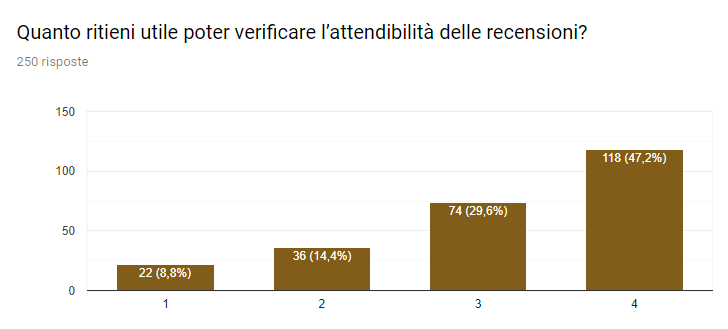
\includegraphics[width=1.0\textwidth]{images/charts-questionario/chart-verifica-recensioni.png}
\end{figure}
\pagebreak
\subsection{Approfondimento task Visita di Gruppo}

A seguito della \textbf{prima revisione} abbiamo effettuato un'ulteriore fase di Needfinding incentrata sul solo task relativo alle \textit{visite di gruppo}.

\paragraph{}
Il numero totale di intervistati è di \textbf{10} persone, e sono sempre studenti della Sapienza. Dalle interviste è emerso che un'organizzazione di visite di gruppo è preferibile tramite un sistema di inviti ben gestito. Inoltre, questo sistema, dovrebbe essere gestito internamente all'applicazione poiché, gli intervistati, ci hanno detto che su applicazioni di messaggistica, come WhatsApp o Telegram, si perdono le informazioni importanti tra i vari messaggi.
\newline
Altrettanto importante è avere una breve descrizione riguardante la mostra o il museo, con relativi orari e luoghi d'incontro, i partecipanti alla visita e i prezzi del biglietto.

\paragraph{}
Da sottolineare il fatto che le risposte delle persone intervistate sono sempre state molto omogenee tra loro, senza grandi contraddizioni.
\pagebreak

\section{Storyboards}

Dopo la fase di Needfinding abbiamo scelto \textbf{4 task} su cui concentrarci:
\begin{itemize}
    \item \textit{Selezione  Preferenze};
    \item \textit{Ricerca con Filtri};
    \item \textit{Notifica} (in base agli interessi);
    \item \textit{Unione a Visita di Gruppo}.
\end{itemize}

\subsection{Selezione Preferenze}

\begin{figure}[h]
    \centering
    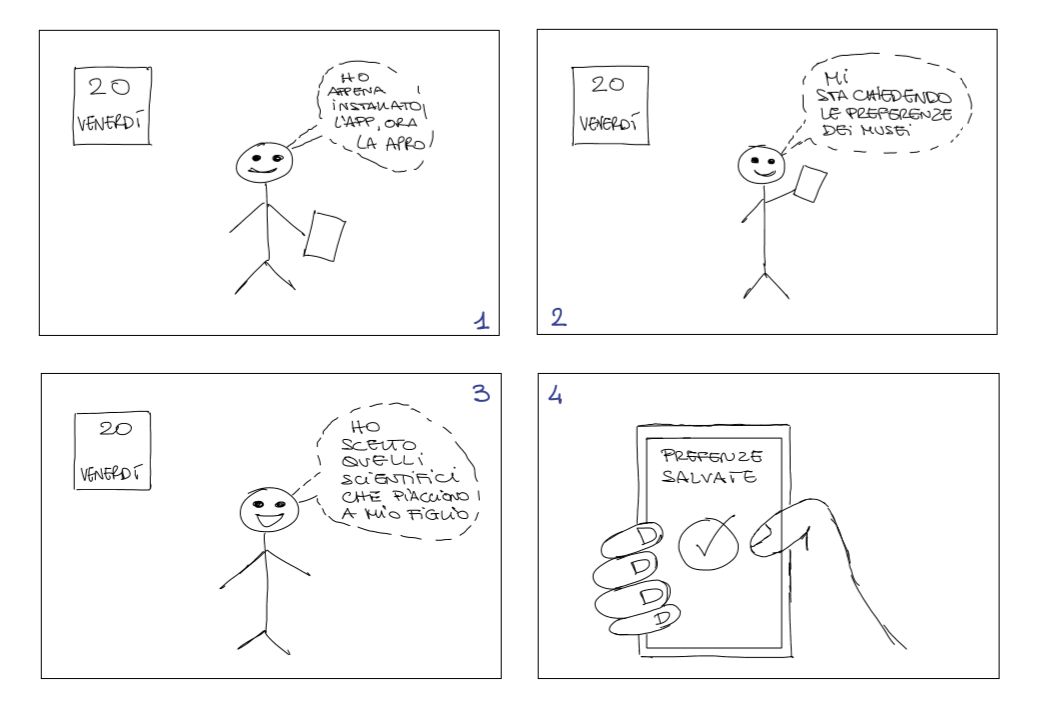
\includegraphics[width=1.0\textwidth]{images/storyboards/Storyboard-1-scelta-preferenze-notitle.png}
\end{figure}

\newpage

\subsection{Ricerca con Filtri}

\begin{figure}[h]
    \centering
    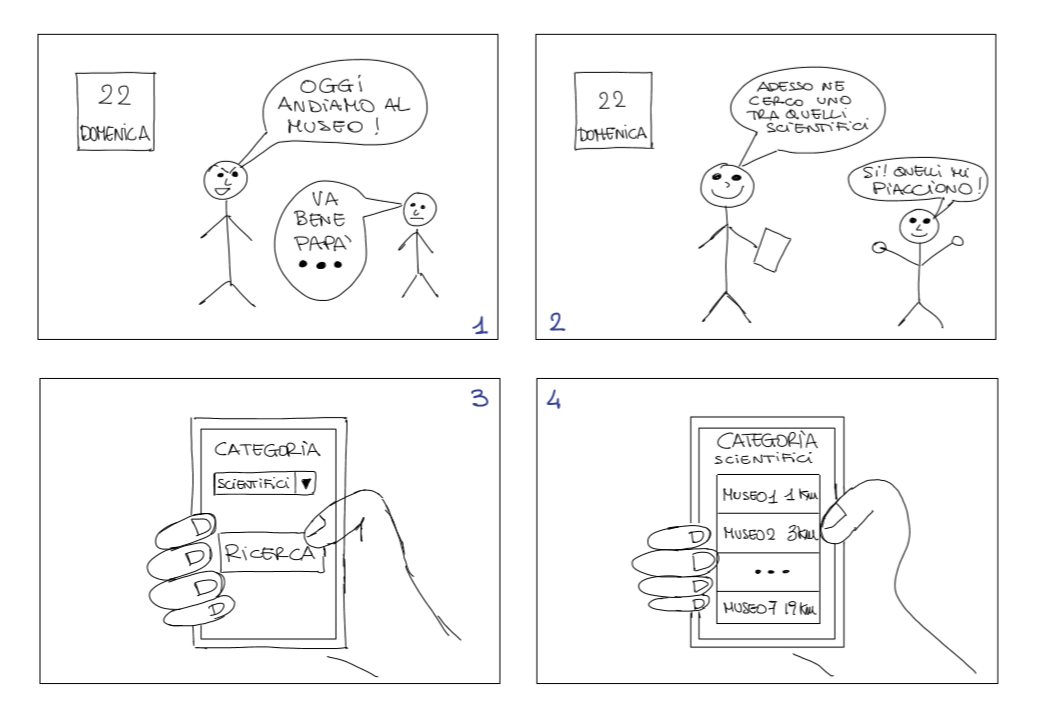
\includegraphics[width=1.0\textwidth]{images/storyboards/Storyboard-2-ricerca-notitle.png}
\end{figure}

\newpage

\subsection{Notifica}

\begin{figure}[h]
    \centering
    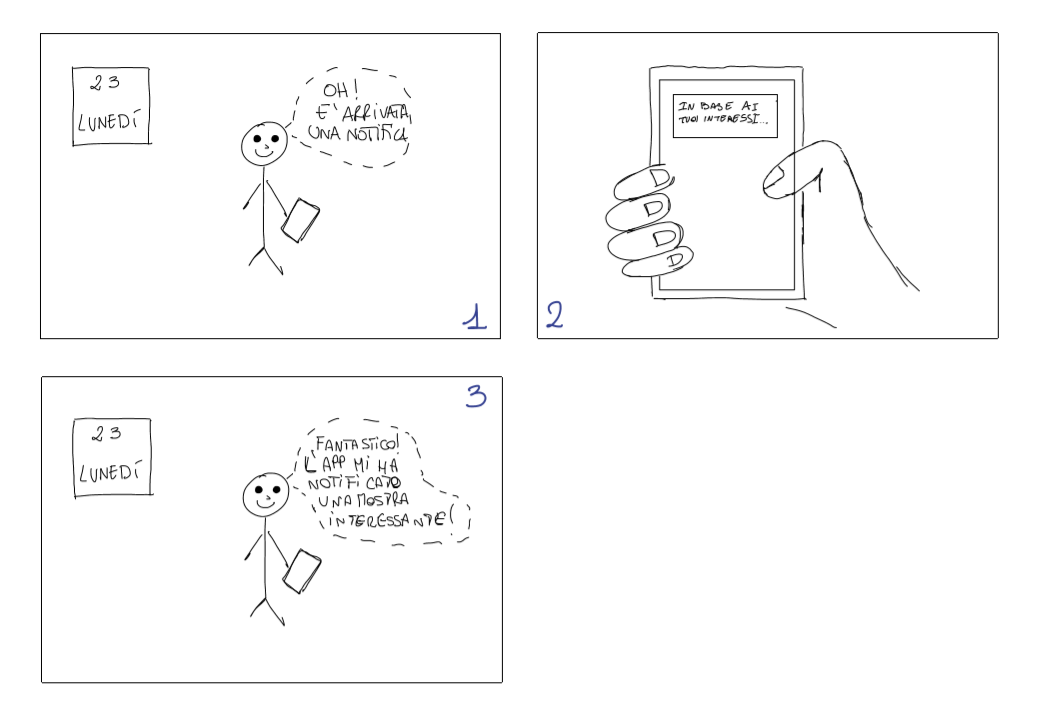
\includegraphics[width=1.0\textwidth]{images/storyboards/Storyboard-3-notifica-notitle.png}
\end{figure}

\newpage

\subsection{Unione a Visita di Gruppo}

\begin{figure}[h]
    \centering
    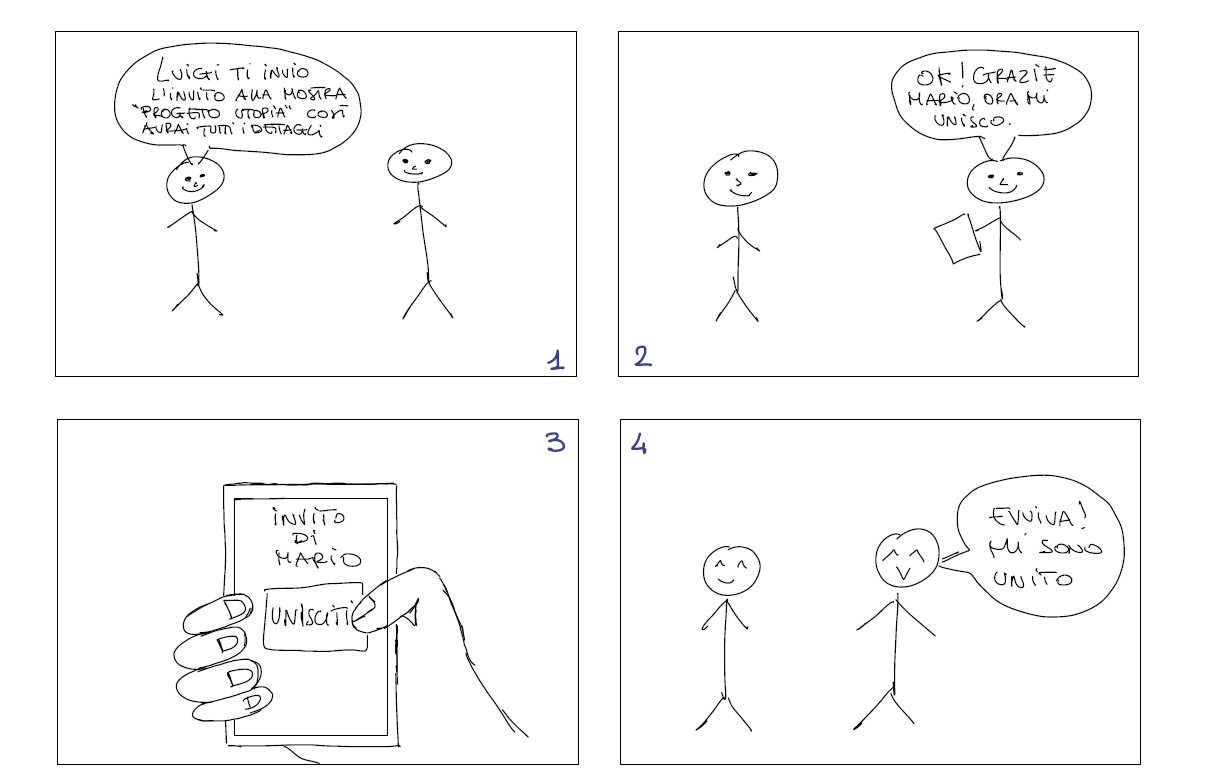
\includegraphics[width=1.0\textwidth]{images/storyboards/Storyboard-4-unione-gruppo-notitle.png}
\end{figure}
\pagebreak

\section{Prototyping}

\subsection{Introduzione}
Il prototipo Marvel è stato creato con \textbf{Android} come piattaforma di riferimento e comprende i seguenti task:
\begin{itemize}
    \item \textit{Selezione  Preferenze};
    \item \textit{Ricerca con Filtri};
    \item \textit{Notifica} (in base agli interessi);
    \item \textit{Unione a Visita di Gruppo}.
\end{itemize}

Il prototipo è stato sviluppato attraverso un approccio \textbf{Incrementale} ed \textbf{Evolutivo}. Abbiamo quindi aggiunto i task al prototipo uno per volta, cominciando da subito con gli \textit{user test}. In base ai risultati dei test è stato deciso ogni volta se effettuare un'ulteriore iterazione per migliorare il prototipo del singolo task o se fosse possibile procedere direttamente al successivo (nel caso non fossero stati riscontrati problemi). 

\paragraph{}
Durante le fasi di test abbiamo utilizzato la tecnica del \textbf{Think Aloud}, chiedendo ad ogni utente di descrivere passo passo le azioni che avrebbero svolto e di dire che cosa pensavano durante il test stesso. Gli utenti selezionati per i test sono stati \textbf{4} e son stati sempre gli stessi.

\subsection{Iterazioni}
Le iterazioni seguenti rappresentano le fasi di prototipazione che abbiamo effettuato. A seguito di ognuna di esse sono stati effettuati gli \textit{user test}, così da poterne valutare i risultati e procedere con un'ulteriore iterazione.

\subsubsection{Iterazione 1}
In questa iterazione abbiamo implementato il task \textbf{Seleziona Preferenze}. Durante i test ci è stato fatto notare che non era possibile evitare di scegliere alcuna preferenza. Inoltre non era chiaro se le preferenze fossero state salvate o meno.

\subsubsection{Iterazione 2}
In questa iterazione abbiamo modificato il task \textbf{Seleziona Preferenze} in base ai risultati dei precedenti test, aggiungendo un bottone \textbf{``SALTA''} e una pagina di conferma dopo la selezione delle proprie preferenze. A seguito di ulteriori test non abbiamo riscontrato alcun problema.

\subsubsection{Iterazione 3}
In questa iterazione è stato implementato il task \textbf{Ricerca con Filtri}.
Grazie agli user test è emerso che non fosse chiaro che per filtrare si dovesse utilizzare il bottone a destra della barra di ricerca.

\subsubsection{Iterazione 4}
In questa iterazione abbiamo modificato il task \textbf{Ricerca con Filtri} in base ai risultati dei precedenti test, aggiungendo una label esplicativa al bottone per selezionare i filtri. A seguito di ulteriori test non abbiamo riscontrato alcun problema.

\subsubsection{Iterazione 5}
In questa iterazione è stato implementato il task \textbf{Notifica}. Durante gli user test non è emerso alcun problema.

\subsubsection{Iterazione 6}
In questa iterazione è stato implementato il task \textbf{Unione a Visita di Gruppo}. Durante gli user test c'è stato solamente fatto notare che il titolo dell'invito riportava solo il nome dell'amico, il che era troppo generico e poteva portare a problemi di omonimia. Oltre a ciò non è emerso alcun problema, abbiamo perciò aggiunto anche il cognome senza effettuare ulteriori test.

\subsection{Seconda revisione}
Durante la seconda revisione sono emersi alcuni problemi da risolvere.

\paragraph{}
Per quanto riguarda il task \textbf{Selezione Preferenze} sarebbe stato preferibile inserire un \textit{dialog di conferma} anziché una pagina di conferma salvataggio preferenze e inoltre la pagina non era raggiungibile dal menù ``hamburger''. 

\paragraph{}
Per quanto riguarda il task \textbf{Ricerca con Filtri} non era ben chiaro quando un filtro fosse attivo o meno. 

\paragraph{}
Per quanto riguarda il task \textbf{Notifica}, poteva risultare poco intuitivo il modo in cui si accede alla Home dopo aver aperto una notifica, abbiamo perciò effettuato nuovamente degli \textit{user test} chiedendo di andare sulla schermata Home per effettuare una ricerca in seguito alla notifica e \textbf{tutti} gli utenti sono riusciti senza difficoltà.

\paragraph{}
Per quanto riguarda l'ultimo task, \textbf{Unione a Visita di Gruppo}, c'erano alcuni problemi: nel menù ``hamburger'' mancava un badge di conteggio inviti ricevuti, gli inviti dovevano avere nel titolo il nome della mostra piuttosto che quello del mittente, il bottone di unione doveva essere più visibile e con un testo differente come ``accetta invito". Infine mancava un collegamento al museo in cui era la mostra.

\subsubsection{Iterazione 7}
In questa iterazione abbiamo modificato il task \textbf{Seleziona Preferenze} inserendo, al posto della schermata unica di conferma, un \textit{dialog} di conferma successivo al tocco del bottone \textit{continua} o \textit{salta}, ed è stato inserito il link al task nel menù ``hamburger''. Durante gli user test non è emerso alcun problema.

\subsubsection{Iterazione 8}
In questa iterazione abbiamo modificato il task \textbf{Ricerca con Filtri}, aggiungendo un colore di background al bottone \textit{filtra} quando un filtro è attivo. Durante gli user test non è emerso alcun problema, e il fatto che il bottone fosse evidenziato quando un filtro era attivo è sempre stato interpretato correttamente.

\subsubsection{Iterazione 9}
In questa iterazione abbiamo modificato il task \textbf{Unione a Visita di Gruppo}. Innanzitutto abbiamo modificato la pagina con la lista inviti mettendo come titolo principale il nome della mostra e come sottotitolo il nome del mittente. Inoltre è stato aggiunto il badge di conteggio inviti in attesa di risposta. Per quanto riguarda le singole card degli inviti, abbiamo reso il titolo cliccabile e abbiamo rimosso il bottone ``informazioni mostra'' per dar più risalto al bottone ``accetta invito''. Durante gli user test gli utenti hanno cliccato correttamente sul titolo della mostra per ottenere le informazioni relative ad essa e non hanno avuto problemi ad accettare l'invito.

\subsubsection{Iterazione 10}
In questa iterazione abbiamo aggiunto la possibilità di ``scrollare'' alcune pagine in quanto durante la maggior parte dei test, seppur non ci sia mai stato fatto presente esplicitamente come problema, abbiamo notato che gli utenti tentavano spesso di scorrere verso il basso per visualizzare più mostre nelle schermate relative alla ricerca o per cercare ulteriori informazioni nelle schermate relative a Mostre o Musei.

\subsection{Link ai prototipi Marvel}
I prototipi realizzati sono consultabili direttamente su Marvel in tre diverse versioni, la prima (1.0) con tutte le modifiche che precedevano la seconda revisione, la seconda (2.0) con tutte le modifiche fatte a seguire della revisione con il professore e la terza (2.1) con le modifiche finali effettuate dopo la prima consegna del progetto:
\begin{enumerate}
    \item[(1.0)] \url{https://marvelapp.com/5g1574g}
    \item[(2.0)] \url{https://marvelapp.com/5gji0j3}
    \item[(2.1)] \url{https://marvelapp.com/541g2b7}
\end{enumerate}

Per accedere direttamente ad ogni singolo task è presente la voce \textit{Opzioni per Sviluppatori (Prototyping)} nel menù ``hamburger'' laterale.

\pagebreak

\section{Conclusioni}

Durante le fasi di Needfinding e di test del prototipo abbiamo riscontrato un grande interesse nel progetto da parte di svariate persone, ricevendo incoraggiamenti e consigli su nuove funzionalità. Il più delle volte questo interesse è stato però ``deluso'' una volta chiarito che non avremmo realizzato l'applicazione finale.

\paragraph{}
Abbiamo quindi pensato di valutare lo sviluppo vero e proprio dell'app una volta terminato il progetto, in quanto ritenuto fattibile da tutti i membri del gruppo e considerato anche che la maggior parte delle tecnologie necessarie sono già conosciute.

\paragraph{}
Per quanto riguarda il database delle mostre e degli inviti questo potrebbe essere creato semplicemente in \textbf{MySQL}. Per avere una reattività immediata tra applicazione, utente e database si potrebbe utilizzare la tecnologia \textbf{WebSocket}, che è sempre più diffusa. In questa maniera si potrebbero mantenere migliaia di utenti connessi contemporaneamente con un unico server. Per quanto riguarda la parte applicazione vera e propria, si potrebbe utilizzare \textbf{React Native} che combina il \textit{nativo} con \textit{React}. Inoltre, alcuni membri del gruppo hanno già esperienza in progetti che utilizzano \textit{javascript} e \textit{React}, ciò permetterebbe di procedere più velocemente nelle prime fasi dello sviluppo, dovendo evitare di approfondire nuove tecnologie da zero.

\end{document}
